\chapter{动力系统基础}\label{chap:dynamic}


\section{动力系统模型概述}
动力系统模型是一种数学工具,用于描述物理系统、生物系统或其他系统随时间演化的行为。它通常基于微分方程或差分方程,通过描述系统内部的状态变量之间的关系来预测系统未来的行为。

动力系统模型可以分为线性模型和非线性模型两种。线性模型假设系统的行为是线性的,通常用线性微分方程或差分方程来描述;而非线性模型则考虑系统的非线性效应,通常需要更复杂的数学形式来描述系统的行为。

\begin{defn}[动力系统]
一个动力系统可以定义为一个状态空间 $\mathcal{X}$ 上的一组微分方程:
\begin{align}
\frac{d\mathbf{x}}{dt} &= \mathbf{f}(\mathbf{x}, t), \quad \mathbf{x} \in \mathcal{X}, \ t \in [0, T]
\end{align}
其中 $\mathbf{x}$ 是状态向量,$\mathbf{f}(\mathbf{x}, t)$ 是系统的动力学方程,$T$ 是观测时间的结束点。
\end{defn}

\begin{defn}[混沌]
    在动力系统模型中,如果系统的状态轨迹表现出无规律、无法预测的行为,并且具有灵敏的初始条件依赖性,那么我们称这种状态为混沌。
\end{defn}

当出现混沌时,一个看似简单的确定性系统可能会表现出极不稳定的动力学行为,这种情况下我们很难进行预测,并且微小的误差可能导致结果有很大的不同,因此在使用动力系统模型进行预测时,我们需要特别注意混沌现象的出现。混沌现象的出现同时跟选择的模型以及参数范围有关。

\begin{defn}[不动点]
    在动力系统模型中,如果存在一个状态 $\mathbf{x}^*$,使得 $\mathbf{f}(\mathbf{x}^*, t) = 0$,那么我们称这个状态为不动点。
\end{defn}

由于在非线性系统中研究不动点的性质往往比较困难,因此我们通常会考虑一些线性化方法来研究不动点的特性。

考虑系统
\begin{equation}
    \begin{aligned}
        \dot{x}=f(x,y)\\
        \dot{y}=g(x,y)
    \end{aligned}
\end{equation}
假定$(x^*,y^*)$为该系统的一个不动点,通过泰勒展开我们可以得到
\begin{equation}\label{0}
    \begin{pmatrix}
        \dot{u}\\
        \dot{v}
    \end{pmatrix}=
    \begin{pmatrix}
        \frac{\partial f}{\partial x} & \frac{\partial f}{\partial y}\\
        \frac{\partial g}{\partial x} & \frac{\partial g}{\partial y}
    \end{pmatrix}_{(x^*,y^*)}\begin{pmatrix}
        u\\ v
    \end{pmatrix}+\text{二次项}
\end{equation}
其中$(u,v)$为$(x^*,y^*)$处的微小扰动,我们将(\ref{0})中去除二次项的部分称为线性化的系统。
\begin{prop}
    在二维动力系统中,在不动点处线性化的动力系统,只要不动点不在边界处,那么该线性化动力系统的不动点性质与原动力系统相同。
\end{prop}

也就是说如果在线性表达式中可以证明不动点是一个吸引子,那么对于原非线性动力系统,该动力系统也是一个吸引子,具体证明可以参考文献\cite{andronov1974qualitative}。
\begin{defn}[吸引子]
    在动力系统中,如果某一状态或状态集合的邻域内的所有轨迹最终都趋近于该状态或状态集合,则该状态或状态集合称为吸引子。
\end{defn}
    
\begin{defn}[极限环]
    极限环是一个孤立的闭轨迹, 孤立意味着它附近的轨迹不是闭的,它们盘旋着靠近或原理极限环。如果当时间$t\to +\infty$ 时,所有的邻近轨迹都趋近于极限环,那么所在的流形被称为稳定的,或者称极限环是稳定的(吸引的)。反之,如果$t\to +\infty$ 时,所有的邻近轨迹都远离于极限环,那么称流形是不稳定的或者极限环是不稳定的(非吸引的)。在所有其它情况下,流形既不是稳定也不是不稳定的,或者称极限环是半稳定的。
\end{defn}

\begin{figure}[H]
    \centering
    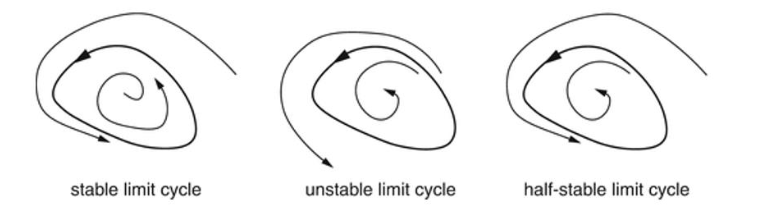
\includegraphics[width=0.8\textwidth]{Img/limit_cycle.png}
    \caption{从左往右依次为稳定极限环,不稳定极限环和半稳定极限环。}
    \label{fig:limit_cycle}
\end{figure}

如图\ref{fig:limit_cycle},极限环分为三种稳定极限环,不稳定极限环和半稳定极限环。稳定极限环是一个吸引子,不稳定极限环是一个排斥子。

稳定极限环模拟了具有自发维持的振荡系统, 如果系统有轻微的扰动,它会自动恢复到标准周期。

\begin{thm}[庞加莱-本迪克松(Poincaré-Bendixson)定理]
    假设:
    \begin{enumerate}
        \item $R$是平面上一个有界闭集;
        \item 有一个定义在包含$R$的开集上的二维动力系统 $\frac{dx}{dt} = f(x, y)$,$\frac{dy}{dt} = g(x, y)$,其中 $f(x, y)$ 和 $g(x, y)$ 是关于状态变量 $x$ 和 $y$ 的实值连续可微函数;
        \item $R$不包含任何不动点;
        \item 存在一个开始于$R$并永远在$R$内运动的轨迹$C$;
    \end{enumerate}
    那么,$R$内的轨迹$C$要么是一个闭轨道,要么当$t \to \infty$时它盘旋靠近一条闭轨道。
\end{thm}

关于证明细节,可以参考Perko(1991)、Coddington和Levinson(1995)的著作,庞加莱-本迪克松定理表明,混沌永远不会在相平面中产生\cite{strogatz2018nonlinear}。

\begin{thm}[Dulac准则]
    令$\frac{d\mathbf{x}}{dt}=\mathbf{f}(\mathbf{x})$是一个定义在平面$R$上一个单连通子集的一个连续可微向量场。如果存在一个定义在相应区域上的实值连续可微函数$g(x, y)$,使得$\nabla \cdot (g \frac{d\mathbf{x}}{dt})$不变号,那么$R$上无闭轨。
\end{thm}
\begin{pf}
    假设有一个闭轨$C$在$R$内,令$A$表示$C$内部的区域,由格林公式可得
    \begin{equation}
        \iint_A \nabla \cdot(g \frac{d\mathbf{x}}{dt})dA=\oint_C g \frac{d\mathbf{x}}{dt}\cdot \mathbf{n}dl
    \end{equation}
    显然左边不等于0, 而右边等于0,这与假设矛盾,所以$R$上无闭轨。
\end{pf}

\section{血糖预测中动力系统模型的发展}
\subsection{葡萄糖动力系统}
在后吸收状态下,葡萄糖由肝脏和肾脏释放到血液中,被体内所有细胞从间质液中移除,并分布到许多生理组分中(例如,动脉血、静脉血、脑脊液、间质液)。我们可以通过以下微分方程来描述葡萄糖动力系统\cite{bergman1979quantitative}:

\begin{equation}\label{1}
    \frac{dG}{dt} = \text{Production} - \text{Uptake},
\end{equation}
其中$G$是血液中的葡萄糖浓度,$t$是时间,Production是葡萄糖生成速率,Uptake是葡萄糖摄取速率(也可以理解为血液中葡萄糖的消耗速率)。

葡萄糖产生和摄取的速率主要取决于血糖和胰岛素水平。这些关系已经通过葡萄糖夹持技术进行了实验定义,该技术允许在各种稳态血糖和胰岛素水平下测量葡萄糖产生和摄取速率\cite{bergman1985assessment}。在恒定胰岛素水平下,葡萄糖产生减少而摄取增加,两者都与血糖水平线性相关\cite{best1981glucose}。这些线性依赖的斜率是“葡萄糖效力”的参数。因此,我们可以将葡萄糖产生和摄取速率表示为:

\begin{equation}\label{2}
    \text{Production} = P_0 -(E_{G0P} + S_{IP} \times I) \times G,
\end{equation}
\begin{equation}\label{3}
    \text{Uptake} = U_0 + (E_{G0U} + S_{IU} \times I) \times G,
\end{equation}

其中$P_0$和$U_0$是零葡萄糖时的葡萄糖产生和摄取速率,\(E_{G0P}\)和\(E_{G0U}\)分别是产生和摄取的零胰岛素葡萄糖效力,\(S_{IP}\)和\(S_{IU}\)分别是产生和摄取的胰岛素敏感性,$I$代表血胰岛素浓度。将方程(\ref{2})和(\ref{3})代入方程(\ref{1}),我们得到

\begin{equation}
    \frac{dG}{dt} = R_0 -(E_{G0} + S_I \times I) \times G,
\end{equation}
其中$R_0$($=P_0-U_0$)是零葡萄糖时葡萄糖的净产生速率,\(E_{G0}\)($=E_{G0p}+E_{G0U}$)是零胰岛素时的总葡萄糖效力,\(S_I\)($=S_{IP}-S_{IU}$)是总胰岛素敏感性\cite{topp2000model}。

再考虑体内的肝糖原水解产生的葡萄糖,最终可以得到
\begin{equation}
    \frac{dG}{dt} = R_0 -(E_{G0} + S_I \times I) \times G+\frac{K_0}{K_1+I^p},
\end{equation}
其中$K_0,K_1,p$为与肝糖原分解产生葡萄糖相关的常数\cite{bridgewater2020amplitude}。
\subsection{胰岛素动力系统}
胰岛素由胰$\beta$细胞分泌,被肝脏、肾脏和胰岛素受体清除,并分布到几个组分中(例如,门静脉、外周血和间质液)。我们可以通过以下微分方程来描述胰岛素动力系统:

\begin{equation}\label{4}
\frac{dI}{dt} = \text{Secretion} - \text{Clearance},
\end{equation}
其中Secretion表示胰岛素分泌速率,Clearance表示胰岛素清楚速率。

我们假设胰岛素清除速率为\(kI\),其中$k$是代表肝脏、肾脏和胰岛素受体中胰岛素摄取的清除常数。

当系统处于近稳态时,胰岛素清除速率与血液胰岛素水平成正比。我们假设胰岛素分泌速率模拟为葡萄糖水平的S形函数\cite{topp2000model}。因此,我们假设

\begin{equation}\label{5}
\text{Secretion} = \frac{\beta\sigma G^2}{(\alpha + G^2)},
\end{equation}

其中$\beta$是胰$\beta$细胞的质量。所有$\beta$细胞被假定以相同的最大速率$\sigma$分泌胰岛素,\(G^2/(\alpha + G^2)\)是一个带有系数$2$的Hill函数,描述了从$0$到$1$的S形范围,在$G=\alpha^{\frac{1}{2}}$时达到其最大值的一半。将方程(\ref{5})代入方程(\ref{4}),我们得到控制胰岛素动力学的方程:

\begin{equation}
    \frac{dI}{dt} = \frac{\beta\sigma G^2}{(\alpha + G^2)} - kI.
\end{equation}

\subsection{胰\(\beta\)细胞动力系统}
尽管胰$\beta$细胞在胰腺中分布复杂,但$\beta$细胞质量动态可以用单一组分模型定量化,新的$\beta$细胞可以通过现有$\beta$细胞的复制、新生(干细胞的复制和分化)和其他细胞的转分化来形成。目前,无法量化新生和转分化的速率。然而,除了在发育期间和在极端生理或化学诱导创伤反应中,这些可以忽略不计\cite{finegood1995dynamics}。基于这些原因,新生和转分化未纳入当前模型,且生成的$\beta$细胞被假定等于所有复制的$\beta$细胞。

我们可以通过以下微分方程来描述胰$\beta$细胞动力系统:
\begin{equation}
    \frac{d\beta}{dt} = (-d_0+r_1G-r_2G^2)\beta,
\end{equation}
其中$d_0$是零血糖时$\beta$细胞的自然死亡率,$r_1$和$r_2$是两个常系数\cite{topp2000model}。
\section{模型分析}

由于胰$\beta$细胞数量变化较慢(一般以天为单位观测),在实时血糖监测的过程中,我们以每次进食为数据分段标准,因此我们可以考虑将$\beta$细胞视为常量,仅考虑葡萄糖-胰岛素动力系统\cite{huard2022mathematical}。我们可以得到如下动力系统模型:
\begin{equation}\label{11}
    \begin{aligned}
        \dot{G} &= a_0-a_1G-a_2GI+\frac{a_3}{a_4+I^p} \\
        \dot{I} &= \frac{b_1 G^2}{G^2 + b_2^2} - b_3 I
    \end{aligned}
\end{equation}
\begin{prop}
    动力系统(\ref{11})有唯一不动点,且该不动点为吸引子
\end{prop}

\begin{pf}
    为寻找该动力系统不动点,我们考查
\begin{equation}
    a_0-a_1G^*-a_2G^*I^*+\frac{a_3}{a_4+(I^*)^p}= \frac{b_1 (G^*)^2}{(G^*)^2 + b_2^2} - b_3 I^*=0
\end{equation}
可以注意到$G^*$越大,$I^*$越大,令
\begin{equation}
    h(G)=a_0-a_1G-a_2G\frac{b_1G^2}{b_3(G^2+b_2^2)}+\frac{a_3(b_3^p(G^2+b_2^2)^p)}{a_4(b_3^p(G^2+b_2^2)^p+b_1^pG^{2p})}
\end{equation}
可以得出$h(G)$单调递减,且$h(0)>0,\lim_{G\to\infty}h(G)<0$,易得$\exists !G^*$使得$h(G^*)=0$因此,动力系统(\ref{11})有唯一不动点。

在点$(G^*,I^*)$处线性化动力系统(\ref{11})可得 
\begin{equation}\label{14}
    \begin{pmatrix}
        \dot{G}\\
        \dot{I}
    \end{pmatrix}=\begin{pmatrix}
        -a_1-a_2I^* & -a_2G^*-\frac{pa_3(I^*)^{p-1}}{(a_4+(I^*)^p)^2}\\
        \frac{2b_1b_2^2G^*}{((G^*)^2 + b_2^2)^2} & -b_3
    \end{pmatrix}\begin{pmatrix}
        G\\
        I
    \end{pmatrix}
\end{equation}
线性动力系统(\ref{14})的特征多项式为$\lambda^2+c_1\lambda+c_2$,其中
\begin{equation*}
    c_1=a_1+a_2I^*+b_3>0, c_2=(a_1+a_2I^*)b_3+\frac{2b_1b_2^2G^*}{((G^*)^2 + b_2^2)^2}(a_2G^*+\frac{pa_3(I^*)^{p-1}}{(a_4+(I^*)^p)^2})>0
\end{equation*}
两个特征值均有负实部,唯一不动点$(G^*,I^*)$为吸引子\cite{strogatz2018nonlinear}。

\end{pf}
\begin{prop}\label{prop2}
    动力系统(\ref{11})全局渐近稳定(即有稳定极限环)
\end{prop}
\begin{pf}
    考虑$g(G,I)=\frac{1}{I}$, 我们有
    \begin{equation}
        \nabla\cdot(g(\dot{G},\dot{I}))=\frac{-a_1}{I}-a_2-\frac{b_1 G^2}{I^2(G^2 + b_2^2)}<0
    \end{equation}
    由Dulac准则,(\ref{11})在$(0,+\infty)\times (0,+\infty)$中无闭轨,由于葡萄糖和胰岛素的值恒大于$0$, 由庞加莱-本迪克松定理知(\ref{11})有稳定极限环,该极限环为唯一不动点$(G^*,I^*)$
\end{pf}

\section{模型参数估计方法}
在实际应用中,我们需要根据实验数据估计模型参数。在估计模型参数时,我们通常使用最小二乘法来拟合模型。最小二乘法是一种常用的参数估计方法,它通过最小化实际观测值和模型预测值之间的残差平方和来估计模型参数。

\begin{defn}[最小二乘法]
    给定一组实验数据$(x_i, y_i)$,我们的目标是找到一组参数$\theta$,使得模型预测值$f(x_i, \theta)$与实际观测值$y_i$之间的残差平方和最小。最小二乘法的目标函数为:
    \begin{equation}
        \theta^* = \arg\min_{\theta} \sum_{i=1}^{n} (y_i - f(x_i, \theta))^2
    \end{equation}
\end{defn}

在实际应用中,我们通常使用数值优化算法来求解最小二乘问题。常用的数值优化算法包括梯度下降法、共轭梯度法、牛顿法等。这些算法可以有效地求解高维非线性最小二乘问题,帮助我们估计模型参数。

我们先将动力系统模型(\ref{11})转化为差分方程形式,然后根据实验数据使用最小二乘法估计模型参数。具体步骤如下:

\begin{enumerate}
    \item 将动力系统模型(\ref{11})转化为差分方程形式:
    \begin{equation}
        \begin{aligned}
            G_{t+1} &= G_{t-1} + 2\Delta t \left(a_0-a_1G_t-a_2G_tI_t+\frac{a_3}{a_4+I_t^p}\right) \\
            I_{t+1} &= I_{t-1} + 2\Delta t \left(\frac{b_1 G_t^2}{G_t^2 + b_2^2} - b_3 I_t\right)
        \end{aligned}
    \end{equation}
    \item 以每次进食为一个阶段将同一个人的数据分为$(G_{ij}, t_{ij})$,其中$j$表示第j阶段进食,通过差分方程算出来的葡萄糖数值为$f(\theta)$,定义损失函数:
    \begin{equation}
        L(\theta) = \sum_{j=1}^{m} \Vert \mathbf{G_j}-f(\theta) \Vert_2^2+\epsilon\Vert \theta \Vert_2
    \end{equation}
    其中$\epsilon$是正则化参数,用于防止过拟合。
    \item 由命题\ref{prop2},我们可以保证模型参数估计的稳定性和收敛性。因此我们可以直接使用梯度下降法求解。
    \begin{equation}
        \theta^* = \arg\min_{\theta} L(\theta)
    \end{equation}
\end{enumerate}